\documentclass[a4paper, 12pt]{article}
\linespread{1.25}
\usepackage{ngerman}
\usepackage[utf8]{inputenc}
\usepackage{amsmath}
\usepackage{amssymb}
\usepackage{dsfont}
\usepackage{graphicx}
\usepackage{subfigure}
\usepackage{float}
\usepackage{anysize}
\usepackage{icomma}
\usepackage[german]{cleveref}
\usepackage[left=2.5cm, right=2.5cm, top=2cm, bottom=2cm]{geometry}
\usepackage{listings}
\usepackage{siunitx}
\usepackage{textcomp}
%\usepackage{caption}
%\usepackage{subfigure}
\crefname{figure}{Abbildung}{Abbildungen}
\crefname{subfigure}{Abbildung}{Abbildungen}

\begin{document}
\title{
\textbf{Computatinal Physics\\
Übung}
}
\date{}
\maketitle

\begin{center}
Jan Doersch, Sebastian Jäger und Leonard Wollenberg\\
Abgabe: 29.04.2016\\
\end{center}
% !TeX root = Notizen.tex

\section*{Aufgabe1: Doppelpendel}
\subsection*{a)}
\newpage
% !TeX root = ../Notizen.tex

\section*{Aufgabe 2: Harmonischer Oszillator}
\subsection*{a)}
Hier wird das Programm aus Aufgabe 1 getestet.
Dazu wird der harmonische Oszillator behandelt, bei dem gilt:
\begin{align}
	\frac{1}{m}\vec{F}(\vec{r})=-\vec{r}~.
\end{align}
Die Anfangsbedingungen werden zunächst als
\begin{align}
	\vec{r}_0&=10\cdot\vec{e}_x~,\\ \vec{v}_0&=\vec{0}
\end{align}
festgelegt und es wird eine Breite von $h=0,1$ im Zeitintervall $t\in[0,\,10]\,\text{s}$ verwendet.\\
\begin{figure}[h!]
	\centering
	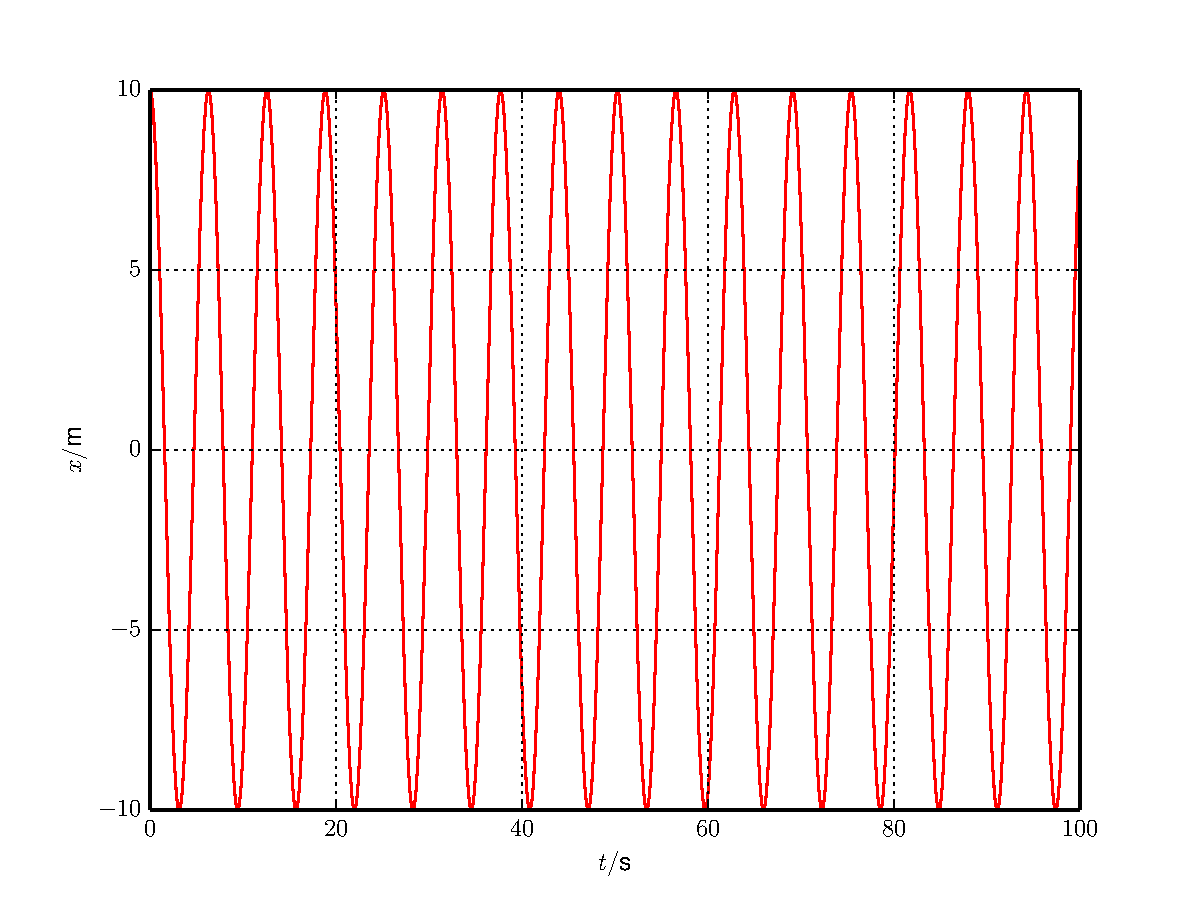
\includegraphics[width = 0.75\textwidth]{../Plots/Plot_2_A_1.pdf}
	\caption{Ergebnis für die Ortskoordinate $x(t)$ für den harmonischen Oszillator.\label{fig:Zentral_X}}
\end{figure}\\
In \cref{fig:Zentral_X} ist die Lösung für $x(t)$ dargestellt.
Sie hat die Form einer harmonischen Schwingung.\\
\newpage
Nun wird der Fall
\begin{align}
	\vec{r}_1&=10\cdot\vec{e}_x~,\\ \vec{v}_2&=10\cdot\vec{e}_y
\end{align}
betrachtet.
\begin{figure}
	\centering
	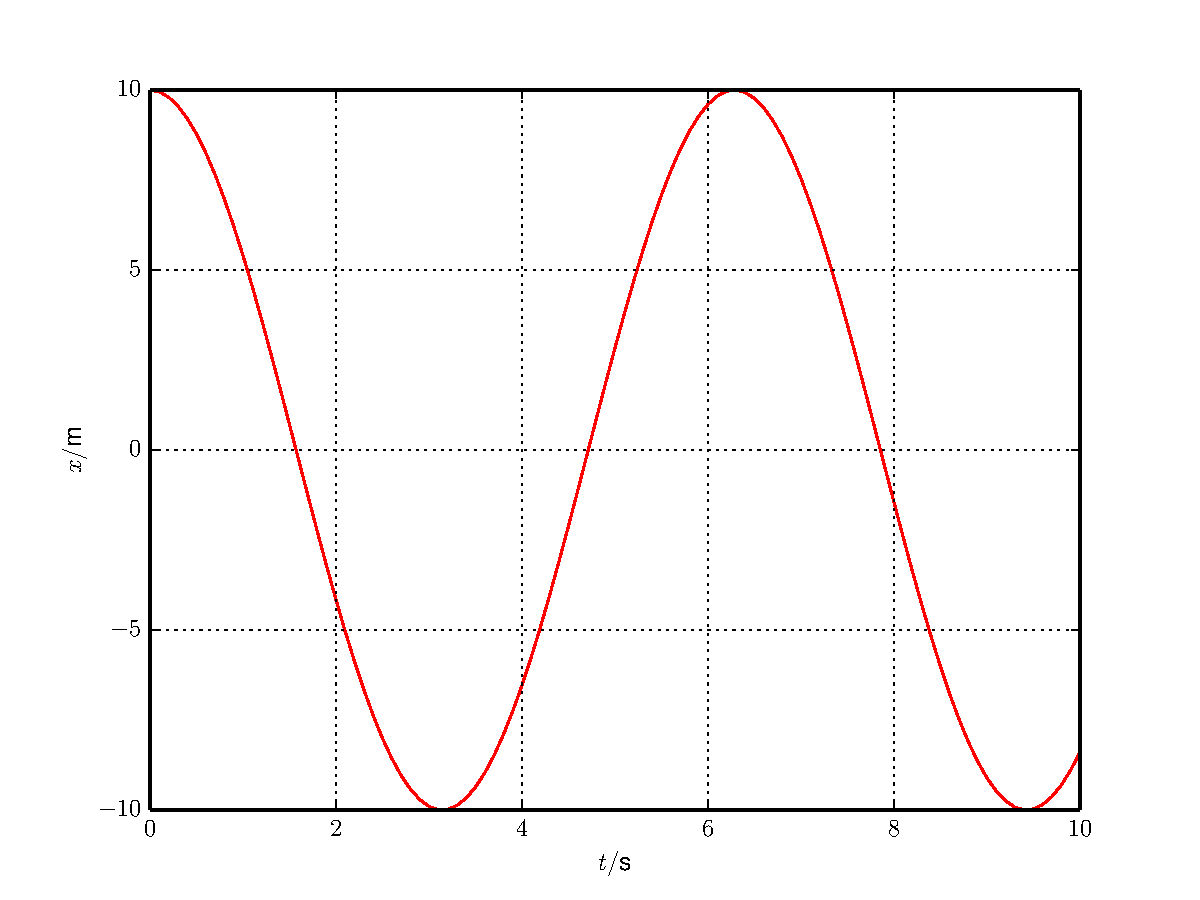
\includegraphics[width = 0.49\textwidth]{../Plots/Plot_2_A_3}
		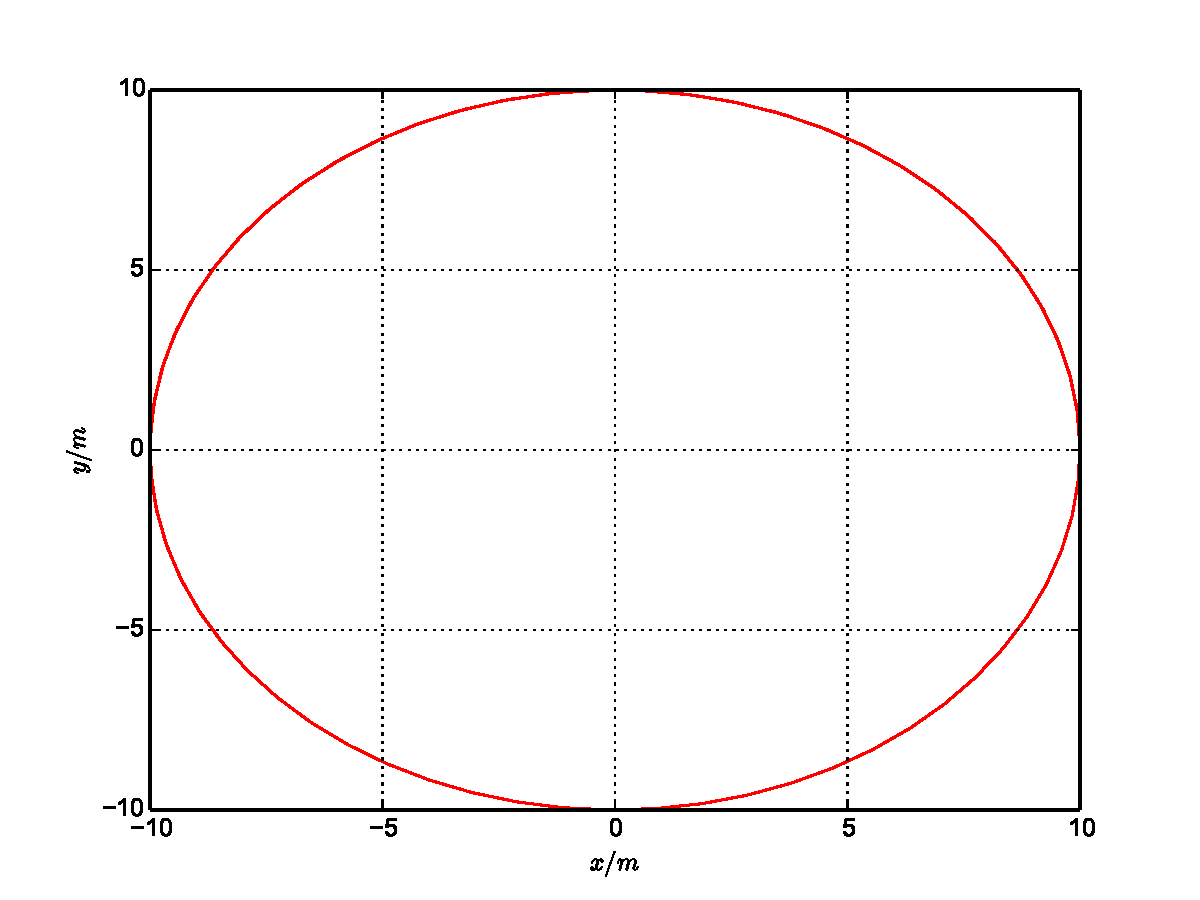
\includegraphics[width = 0.49\textwidth]{../Plots/Plot_2_A_2}
		\caption{Lösung für die Ortskoordinate $x(t)$ (links) und Lösung für den Ortsvektor $\vec{r}(t)$ für den harmonischen Oszillator mit $\vec{r}_1$ und $\vec{v}_1$ (rechts).\label{fig:Geschw}}
\end{figure}
Es lässt sich in \cref{fig:Geschw} erkennen, dass $x(t)$ wieder eine harmonische Schwingung darstellt und $\vec{r}(t)$ eine harmonische Schwingung um den Koordinatenursprung ergibt.
\newpage

\subsection*{b)}
Hier wird überprüft, ob die Energie in dem simulierten System erhalten ist.
Dazu wird die Energiedifferenz $\Delta E= |E(t_n)-E(t_{n-1})|$ bestimmt.
Dabei gilt für die Energie
\begin{align}
	E = T + V =& \frac{1}{2}m\left( v^2 - \int \vec{F}(\vec{r})\text{d}\vec{r} \right) =\frac{1}{2}m\left( v^2 + r^2 \right) \overset{!}{=} \text{const}\\
	\Rightarrow \Delta E =& 0~.
\end{align}

\begin{figure}[h]
	\centering
	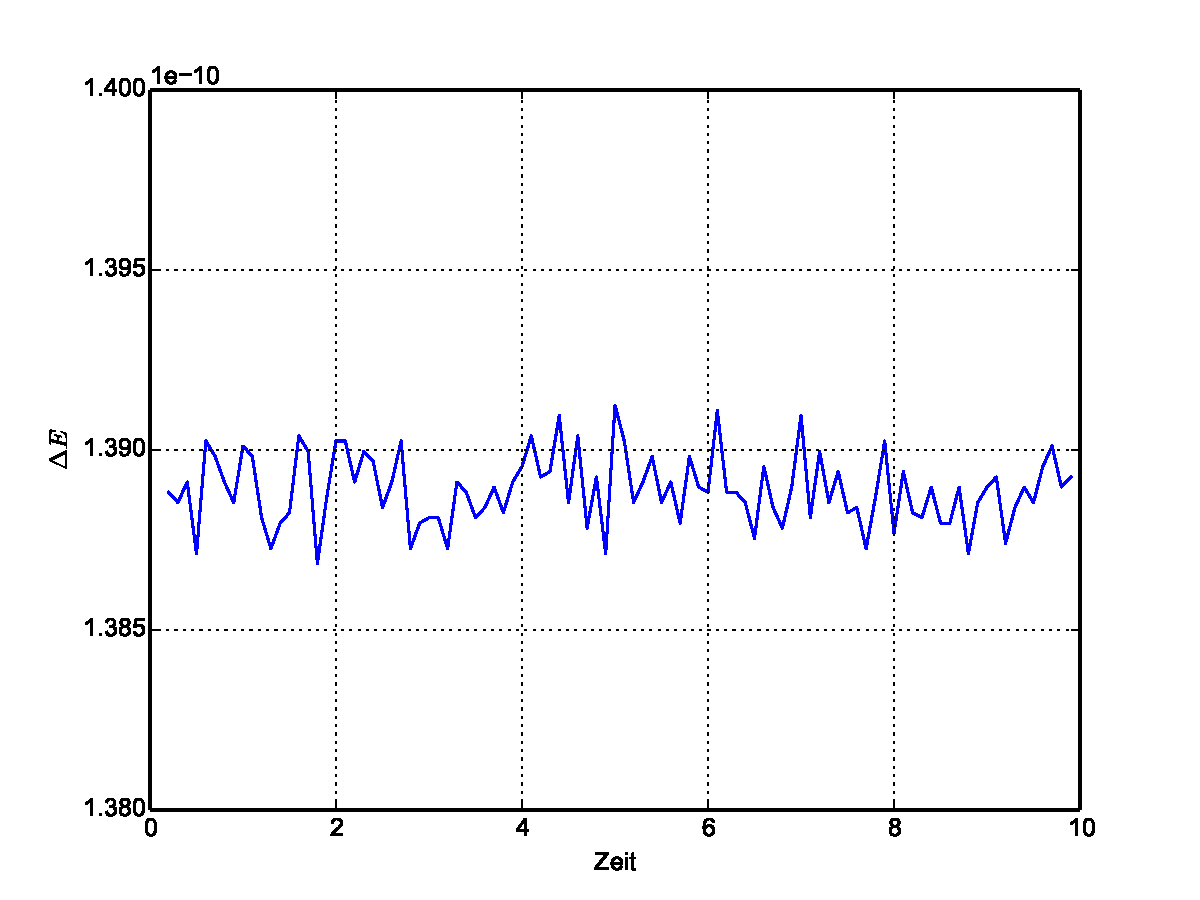
\includegraphics[width = \textwidth]{../Plots/Plot_2_B_Energie.pdf}
	\caption{Energiedifferenz $\Delta E$ für verschiedene Zeiten $t$.\label{fig:EnergieDiff}}
\end{figure}
In \cref{fig:EnergieDiff} ist das Ergebnis dargestellt. Dabei ist darauf zu achten, dass $\Delta E$ mit dem Faktor $10^{-10}$ skaliert.
Der Wert der Energie schwankt also nur sehr leicht und ist mit numerischen Ungenauigkeiten zu erklären.
Es gilt demnach $\Delta E\approx 0$.
\newpage
Um zu überprüfen, welche Größe die Schrittweite $h$ haben muss, damit nach mehreren Oszillationen immer noch die maximale Ausgangsauslenkung erreicht wird, wird im betrachteten Zeitintervall $t\in[0,\,10]\,\text{s}$ das zuletzt erreichte Maximum gesucht.
Dieses ist in \cref{fig:AmplitudeSchritt} gegen die Schrittweite $h$ aufgetragen.
Es zeigt sich, dass bei hohen $h$ z.T. nur nach der ersten Oszillation wieder die Ausgangsauslenkung erreicht wird.
Bei sehr kleinen Auslenkungen hingegen funktioniert das bis mindestens zur siebten Oszillation.
Es ist demnach ratsam, ein $h$ im Bereich zwischen 0,04 und 0,12 zu wählen, denn in diesem Bereich werden sogar häufig noch mehr Oszillationen erreicht.
\begin{figure}[h]
	\centering
	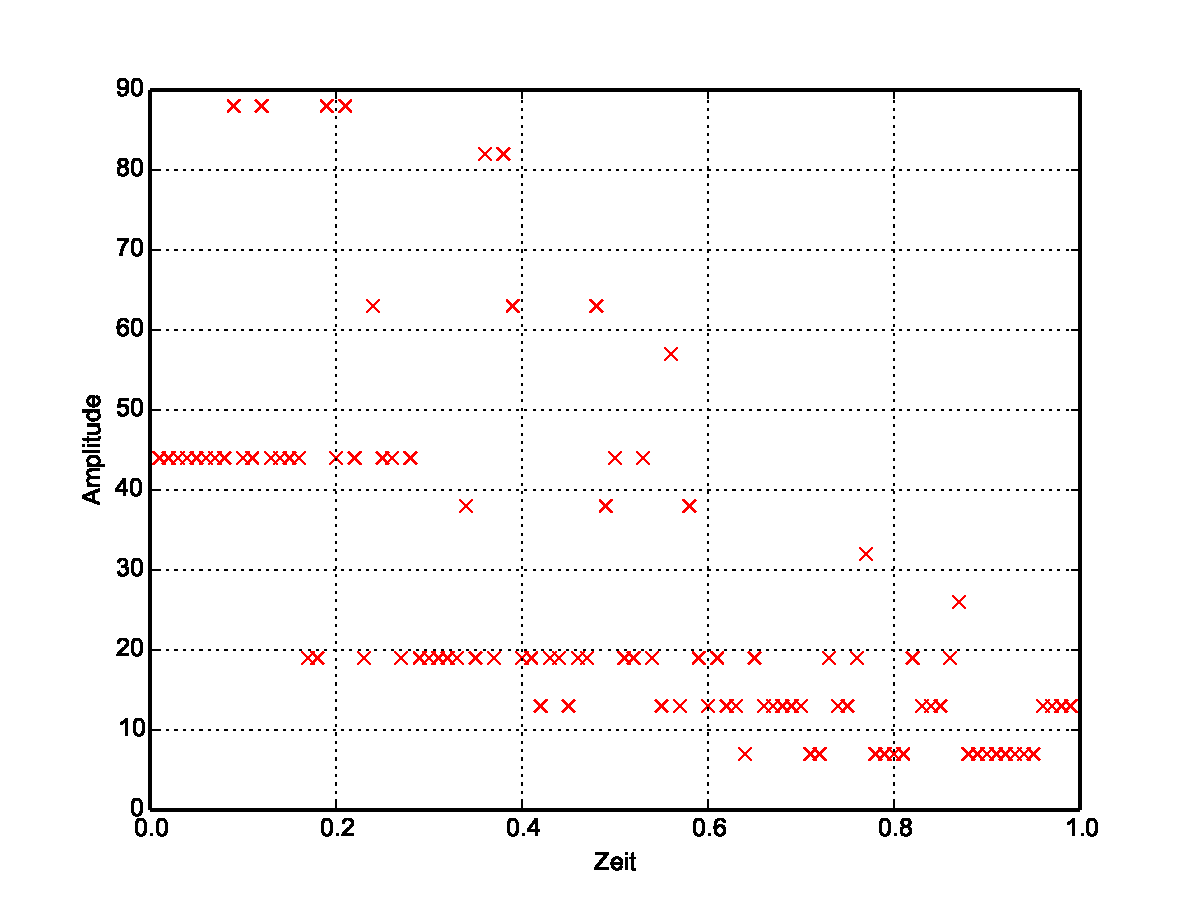
\includegraphics[width = \textwidth]{../Plots/Plot_2_B_Stabilitaet_Zeit.pdf}
	\caption{Zeitpunkt der letzten erreichten Amplitude in Abhängigkeit von der Schrittweite $h$.\label{fig:AmplitudeSchritt}}
\end{figure}\newpage
Der Wert der zuletzt erreichten Amplitude ist in \cref{fig:Stabilitaet} gegen die Schrittweite $h$ aufgetragen.
Hier ist zu sehen, dass die letzte maximale Auslenkung für große $h$ nicht mehr das Ausgangsmaxmimum, den Wert 1, erreicht.
Für eine genauere Betrachtung wird der Bereich bis $h=0,4$ nochmal einzeln dargestellt.
\begin{figure}[H]
	\centering
	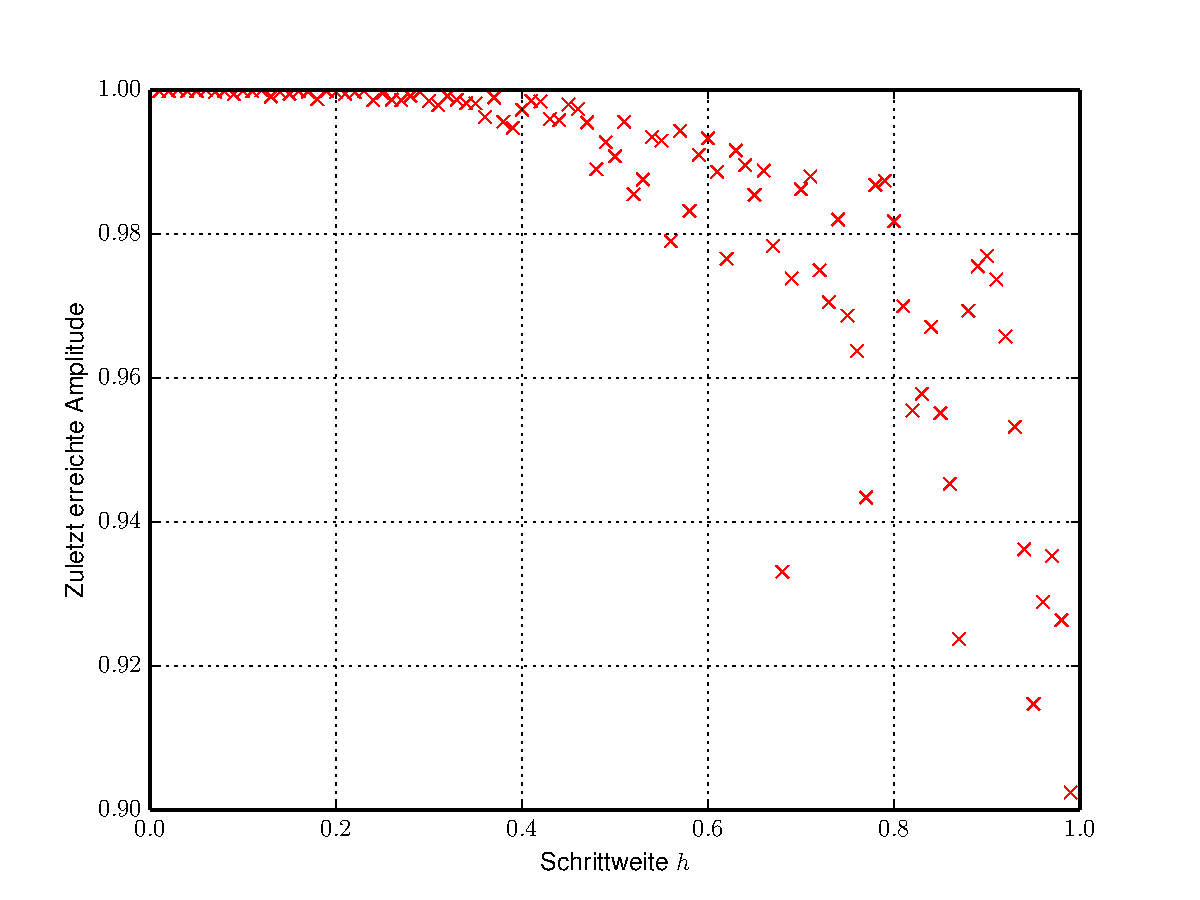
\includegraphics[width = \textwidth]{../Plots/Plot_2_B_Stabilitaet.pdf}
	\caption{Zuletzt erreichte Amplitude in Abhängigkeit von der Schrittweite $h$.\label{fig:Stabilitaet}}
\end{figure}
In \cref{fig:Stabilitaet_Nah} ist nun zu erkennen, dass die Schrittweiten in diesem Bereich auch noch stark streuen, lediglich auf einer kleineren Skala.
Im Bereich bis etwa $h=0,13$ ist die Amplitude allerdings oberhalb vom Wert 0.999, sodass dieser Bereich durch die Amplitudenanalyse insgesamt am ehesten zu empfehlen ist.
\begin{figure}[H]
	\centering
	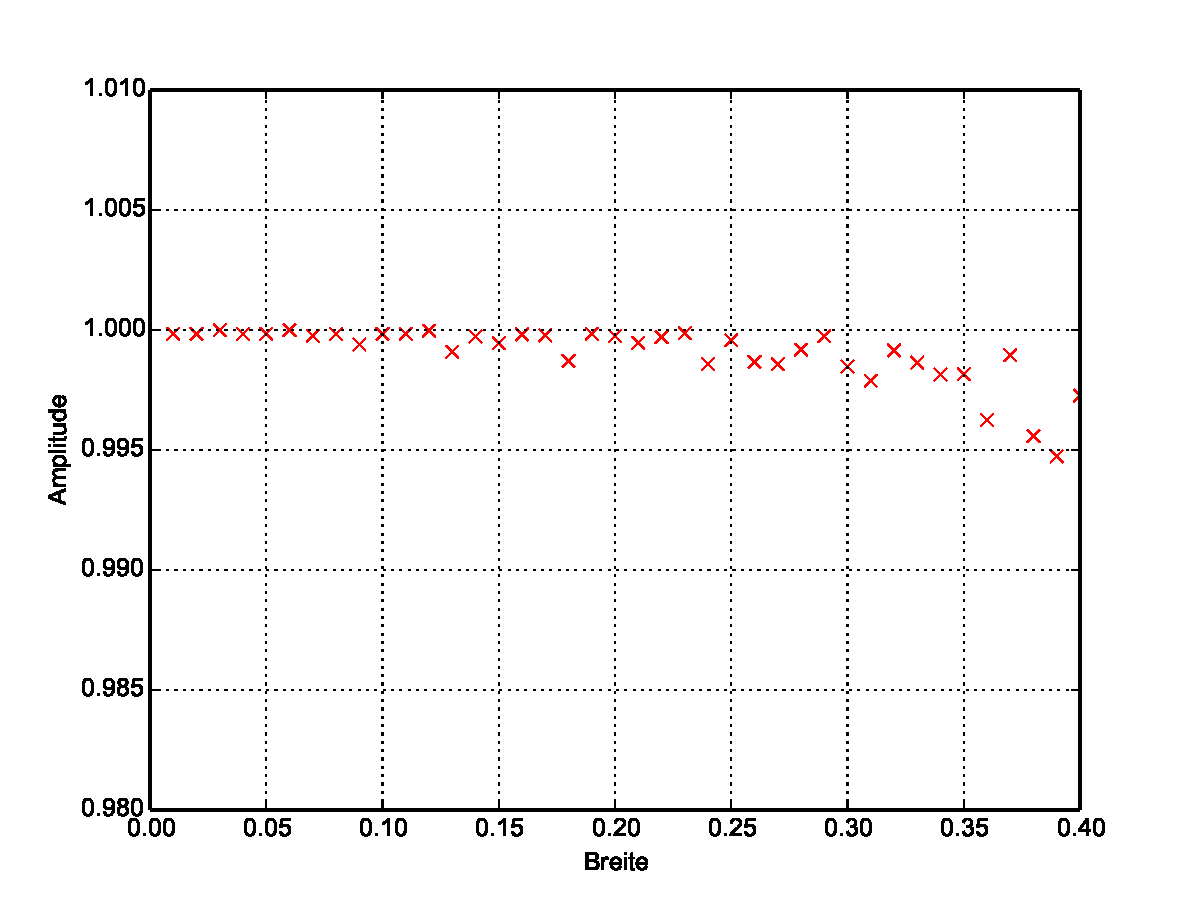
\includegraphics[width = \textwidth]{../Plots/Plot_2_B_Stabilitaet_Nah.pdf}
	\caption{Zuletzt erreichte Amplitude in Abhängigkeit von der Schrittweite $h$.\label{fig:Stabilitaet_Nah}}
\end{figure}
Zusammengefasst lässt sich feststellen, dass sich die Amplitudenbetrachtung und die Betrachtung der Oszillationen im Intervall $h\in[0,04,~0,12]$ überschneiden.
Somit scheint die Wahl einer Schrittweite aus diesem Wertebereich am sinnvollsten.



\end{document} 